

\subsection{L3: Autonomy over Future Learning Experience}
\label{sec:l3-experience-autonomy}

L3 adds autonomy over \emph{what learning experience to acquire next}.
Whereas L2 concerns decisions about how to improve, the additional autonomy
examined at L3 concerns the learning agenda: the system uses evidence about
its current capabilities, failures, and learning history to determine what
it should learn from next.
Learning then changes the state on which subsequent experience acquisition
depends, connecting experience selection and persistent improvement across
rounds.

The characteristic loop at this level can be summarized as follows:

\begin{center}
\fcolorbox{black!25}{gray!4}{%
\begin{minipage}{0.92\linewidth}
\centering
\vspace{6pt}

\LoneStep{observe learner state}
\(\;\longrightarrow\;\)
\LoneStep{choose learning experience}
\(\;\longrightarrow\;\)
\LoneStep{acquire experience}

\par\vspace{7pt}

\(\;\longrightarrow\;\)
\LoneStep{update persistent state}
\(\;\longrightarrow\;\)
\LoneStep{reshape future experience}
\(\;\longrightarrow\;\)
\LoneStep{repeat}

\vspace{6pt}
\end{minipage}%
}
\end{center}

The defining property is \emph{learner-conditioned future experience
acquisition}.
Evidence about the evolving learner must inform a decision about which
experience to select, generate, or seek for subsequent learning, and the
resulting persistent update must feed back into later acquisition decisions.
This decision may be implemented by a separate curriculum component or
integrated into the agent's policy.
A policy update that incidentally changes visited states does not, by itself,
demonstrate autonomy over the learning agenda.

Experience need not be generated from scratch.
Repeatedly selecting material from an externally supplied pool can exhibit
this mechanism when selection adapts to the learner and participates in the
continuing loop; one-time filtering or retention alone does not.
Likewise, the objective, evaluator, update procedure, and rules governing
experience selection may be human-designed.
The relevant distinction is whether learner feedback autonomously changes
the next learning agenda, without requiring a human to redesign it after
each round.
Persistent learning may reside in model parameters or reusable external
state, including memories and skills.

The examples below examine this experience-autonomy mechanism within
particular improvement loops.
Figure~\ref{fig:L3} illustrates two representative realizations of this
feedback structure: adaptive task generation and self-play, and
autonomous practice through environment interaction.
Evidence for this mechanism should be interpreted alongside the other
requirements of the hierarchy when assigning an overall system level.


\begin{figure*}[!t]
    \centering
    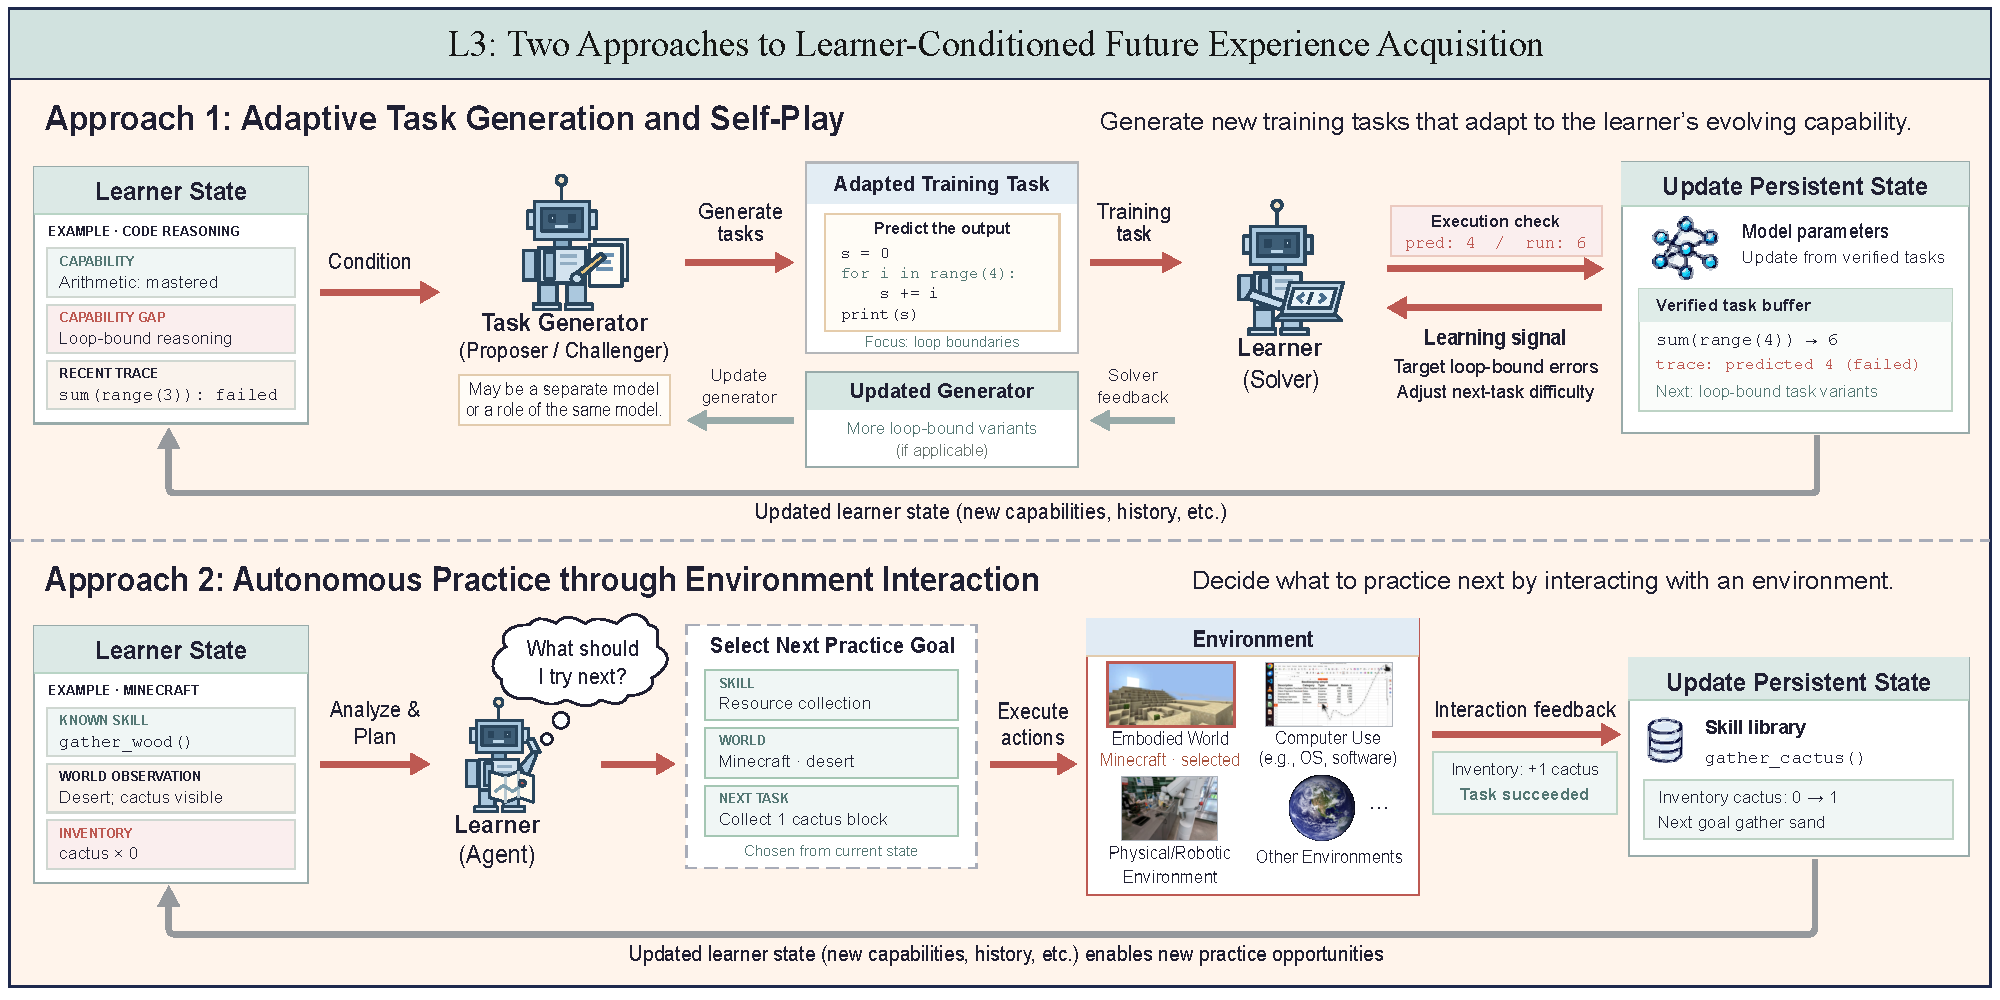
\includegraphics[width=1\linewidth]{figures/L3.pdf}
\caption{Overview of L3: Learner-Conditioned Experience Acquisition.
Under human-defined objectives and evaluation constraints, the system
uses its current capabilities, failures, and interaction history to
determine what to learn from next.
\textbf{Top: Adaptive task generation and self-play.}
A task generator proposes training tasks targeted to the learner's
weaknesses, illustrated by code-reasoning tasks addressing loop-bound
errors. Execution-based feedback supports persistent learner updates
and, where applicable, refinement of the generator.
\textbf{Bottom: Autonomous practice through environment interaction.}
The agent selects a practice goal based on its current skills and
environmental observations, illustrated by collecting cactus in
Minecraft, and consolidates successful experience into a reusable
skill library.
In both approaches, persistent updates reshape subsequent task
generation or practice selection, closing the feedback loop between
learning and future experience acquisition.}    \label{fig:L3}
\end{figure*}



\subsubsection{From Industrial Automation to Experience Autonomy}

\noindent\textbf{Modern training-data pipelines automate many data operations,
but execution automation alone does not establish experience autonomy.}
Drawing on the publicly documented practices reviewed here
~\cite{soldaini2024dolma,young2024yi,qwen2025qwen3,abdin2024phi4},
we organize recurring functions into six components: data-source preparation,
data labeling, data selection, data construction, data mixture and training
orchestration, and model-feedback diagnosis.
These functions need not form a fixed sequence; they can recur across
pretraining, supervised fine-tuning, preference optimization, and
reinforcement learning.

Fig.~\ref{fig:industrial-data-automation} summarizes this landscape
schematically.
Operations such as ingestion, filtering, and sample generation can be
executed at scale once their inputs and acceptance criteria are specified
~\cite{soldaini2024dolma,penedo2024fineweb,qwen2025qwen3}.
The reviewed reports also describe researcher-defined choices concerning
data policies, generation and mixture strategies, training stages, and
experimental evaluation
~\cite{young2024yi,penedo2024fineweb,li2024datacomplm}.
These choices illustrate the distinction between automating an operation
and delegating decisions about the subsequent learning agenda.

\begin{figure}[t]
    \centering
    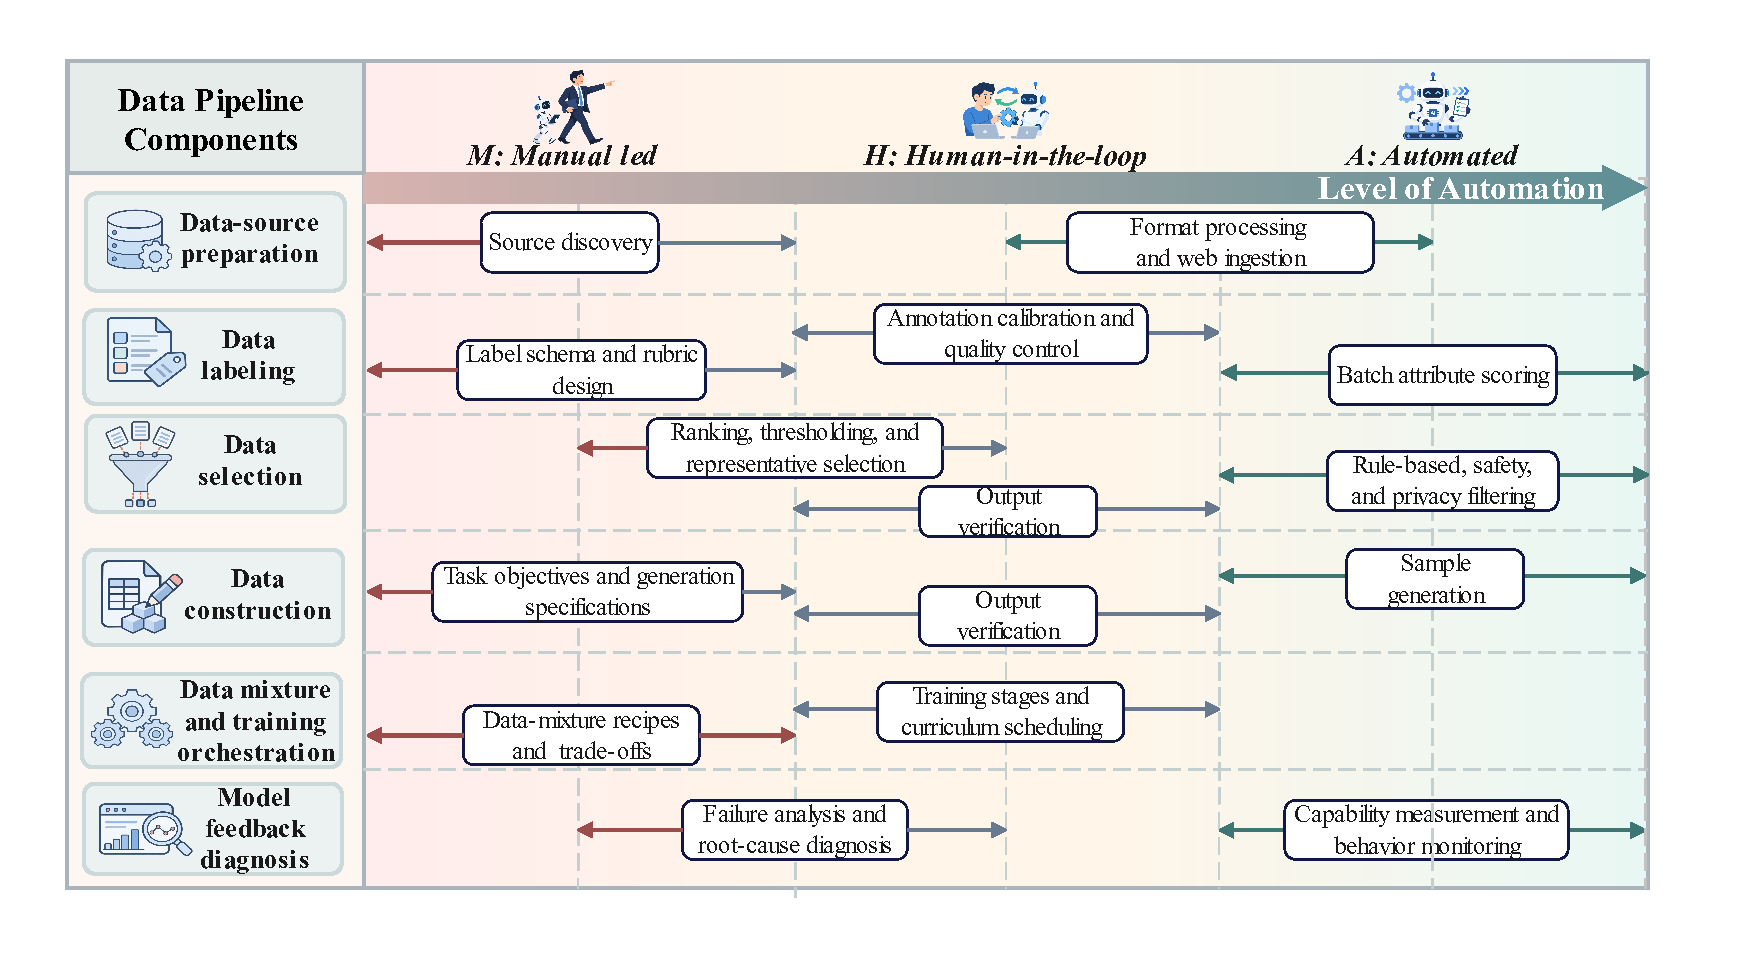
\includegraphics[width=\linewidth]{figures/industrial_data_automation.pdf}
    \caption{Schematic synthesis of automation in the training-data pipelines
    reviewed here. Rows denote six functional components, and rounded bars
    represent recurring operations. Horizontal position indicates a qualitative
    progression from manual-led (M), through human-in-the-loop (H), to automated
    (A). Positions and spans are an interpretive synthesis of reported practices,
    not quantitative measurements or per-organization scores. Operational
    automation is distinct from the additional requirement that learner
    feedback autonomously reshape experience acquisition across learning rounds.}
    \label{fig:industrial-data-automation}
\end{figure}

Human-designed rules do not preclude the L3-specific mechanism.
A fixed selection algorithm can still produce an adaptive learning agenda
if it uses the changing learner's feedback to choose subsequent experience.
Conversely, an automated pipeline that repeatedly generates and filters data
does not establish experience autonomy merely by producing new samples.
The decisive evidence is a closed dependence between learner state,
experience acquisition, persistent learning, and later acquisition decisions.
The pipeline descriptions cited here document substantial operational
automation, but do not by themselves establish this full dependence
~\cite{young2024yi,qwen2025qwen3,abdin2024phi4}.
This evidential distinction does not imply that industrial systems necessarily
lack such mechanisms.

The research examples below illustrate two recurring patterns:
\emph{adaptive task generation and self-play}, and
\emph{autonomous practice through environment interaction}.
They are complementary organizational views rather than exhaustive or
mutually exclusive categories: an interactive agent may also generate its
own tasks, and learner-conditioned selection can operate within either
pattern or over an existing data pool.

Table~\ref{tab:l3-experience-summary} compares representative loops by their
improvement target, learner-conditioned mechanism, and external constraints.

\begin{table*}[t]
\centering
\caption{Representative improvement loops exhibiting learner-conditioned
future experience acquisition. Constraints describe the scope of the
discussed loop, rather than independently establishing a system's maximum
autonomy level.}
\label{tab:l3-experience-summary}
\scriptsize
\setlength{\tabcolsep}{4pt}
\renewcommand{\arraystretch}{1.16}
\begin{tabularx}{\textwidth}{@{}
>{\raggedright\arraybackslash}p{0.12\textwidth}
>{\raggedright\arraybackslash}p{0.13\textwidth}
>{\raggedright\arraybackslash}p{0.39\textwidth}
>{\raggedright\arraybackslash}X
@{}}
\toprule
\textbf{Method}
& \textbf{Target}
& \textbf{Learner-conditioned mechanism}
& \textbf{Externally specified constraints}\\
\midrule
\multicolumn{4}{@{}l}{\textbf{Adaptive Task Generation and Self-Play}}\\
SSP~\cite{lu2026searchselfplay}
& Search agent
& Solver performance shapes proposer rewards and subsequent search tasks.
& Reward design and training procedure.\\
AZR~\cite{zhao2025absolutezero}
& Reasoning model
& Solver-dependent learnability rewards guide executable task proposal.
& Task formats, code executor, and update rules.\\
R-Zero~\cite{huang2026rzero}
& Reasoning model
& Solver answer consistency supplies a proxy that shapes Challenger tasks.
& Uncertainty reward, pseudo-label scheme, and optimization.\\
STP~\cite{dong2025stp}
& Theorem prover
& Conjectures near the current prover's frontier train the conjecturer.
& Formal domain, proof checking, and training rules.\\
PSV~\cite{wilf2026psv}
& Coding model
& Solver-derived difficulty labels condition specification generation.
& Formal verifier, difficulty scheme, and training recipe.\\
VisPlay~\cite{he2026visplay}
& Vision-language model
& Reasoner answer consistency and diversity rewards guide visual questions.
& Image source, reward design, and optimization.\\
\midrule
\multicolumn{4}{@{}l}{\textbf{Autonomous Practice through Environment Interaction}}\\
VOYAGER~\cite{wang2023voyager}
& Embodied agent
& Agent state and exploration history guide objectives; learned skills persist.
& Minecraft interface, curriculum prompts, and skill representation.\\
SIMA 2~\cite{deepmind2025sima2}
& Embodied agent
& In the full ASKA setup, evaluation feedback directs practice toward weaker skills.
& Task setter, reward rubric, and training procedure.\\
SEAgent~\cite{sun2026seagent}
& Computer-use agent
& Trajectory feedback updates a software guidebook that conditions later tasks.
& Software interfaces, assessment model, and learning procedure.\\
\bottomrule
\end{tabularx}
\end{table*}

\subsubsection{Adaptive Task Generation and Self-Play}

\noindent\textbf{The value of a training task changes as the learner improves.}
A fixed task distribution does not explicitly track this moving competence
frontier: familiar tasks may become uninformative, while tasks far beyond
current capabilities may provide little usable learning signal.
Adaptive generation addresses this problem by using learner-dependent
signals to estimate which tasks may support further improvement.
The central challenges are to obtain an informative signal, translate it
into a useful task distribution, and maintain the validity of the resulting
experience.

Search Self-Play (SSP)~\cite{lu2026searchselfplay} connects the first two
challenges by making proposer rewards depend on current solver performance.
As the solver changes, so does the incentive governing future search
problems, allowing the curriculum to evolve without manually redesigning
each task batch.
Absolute Zero Reasoner (AZR)~\cite{zhao2025absolutezero} couples proposal and
solution of executable reasoning tasks within a single model.
Its solver-dependent learnability reward guides task proposal, while a code
executor validates proposed tasks and checks solutions.
This separates two requirements that unconstrained synthesis can conflate:
experience must be evaluable, and its difficulty must be useful for the
current learner.

R-Zero~\cite{huang2026rzero} uses a Challenger--Solver architecture to adapt
task generation without externally supplied answer labels.
The Challenger's uncertainty reward depends on the consistency of multiple
responses from the current Solver; updates to the Solver therefore alter
the signal governing subsequent tasks.
This consistency-based quantity is a proxy for model-perceived difficulty,
not direct evidence of answer correctness or future learning gain.
Its role in the loop is to make experience acquisition responsive to the
learner even when stronger correctness signals are unavailable.

Formal domains provide an alternative route to reliable feedback.
STP~\cite{dong2025stp} addresses sparse proof rewards by jointly developing a
conjecturer and a prover.
Generated conjectures that the current prover can prove only with difficulty
provide training material for the conjecturer, while checked proofs improve
the prover.
The prover's changing frontier thus reshapes subsequent conjectures.
Proof assistants support correctness checking within the formal domain;
the learner-dependent selection criterion serves the separate purpose of
identifying useful training difficulty.

Propose, Solve, Verify (PSV)~\cite{wilf2026psv} brings a related mechanism to
verified code generation.
Solver-derived difficulty labels accompany examples used to prompt new
specifications.
Candidate specifications are checked for compilability, and generated
solutions are formally checked against their specifications before being
used for training.
These checks establish properties relative to the formal specification;
they do not guarantee that the specification expresses a useful task or
that its solution will improve the learner.
Indeed, PSV reports substantial overlap between the realized difficulties
of problems targeted as easy, medium, and hard, showing that
difficulty-conditioned proposal offers partial rather than exact
curriculum control.

VisPlay~\cite{he2026visplay} extends this approach to vision-language
reasoning using an image-conditioned Questioner and a Reasoner.
The Questioner receives an uncertainty reward that favors questions whose
majority-answer confidence is near the prescribed midpoint, together with
a diversity penalty that discourages repetitive questions.
As the Reasoner changes, its response consistency changes the reward for
future question generation.
As in R-Zero, the resulting signal is scalable but can reflect ambiguity
or inconsistent answers as well as productive difficulty.

Across these systems, feedback differs along two connected dimensions.
Executable outcomes and formal proof checking can ground correctness
within a specified task setting, whereas answer consistency estimates
difficulty without independently establishing correctness.
Adaptation may reside in a trained proposer or in generation prompts and
selection procedures conditioned on current learner measurements.
These choices trade off verification scope, feedback cost, and sensitivity
to imperfect proxies.
The shared advance is that estimated learning value influences future
experience acquisition, and persistent learning changes that estimate in
later rounds.

\subsubsection{Autonomous Practice through Environment Interaction}

\noindent\textbf{Interactive agents must decide where to spend their next
learning effort.}
Collecting additional trajectories alone does not resolve this problem:
unguided exploration may revisit mastered behaviors, while a fixed practice
schedule cannot explicitly respond to newly acquired skills or persistent
failures.
The systems below connect interaction feedback to future practice objectives,
using persistent learning to make subsequent experience more responsive to
the agent's changing capabilities.

VOYAGER~\cite{wang2023voyager} combines an automatic curriculum with a
persistent library of executable skills in Minecraft.
Current agent state and exploration history inform new objectives, while
successful behaviors become reusable skills for later tasks.
This couples curriculum decisions to accumulated capability: learning
changes what the agent can attempt, and further exploration supplies
experience from which additional skills can be acquired.
The relevant persistence is in external skills rather than a requirement
to update the underlying language model's parameters.

SIMA 2~\cite{deepmind2025sima2} illustrates why the experimental setting
matters when identifying this mechanism.
Its fixed-task experiment demonstrates improvement from self-generated
trajectories, but does not alone establish autonomy over task selection.
In the full ASKA self-improvement setup, a Gemini-based task setter instead
uses downstream reward-model evaluations to focus practice on weaker skills.
The resulting experience trains the agent, connecting capability assessment
to subsequent practice allocation.
The relevant autonomy belongs to this coupled learning system, including
its task setter, rather than requiring the acting model to make every
curriculum decision itself.

SEAgent~\cite{sun2026seagent} addresses practice in unfamiliar software
through an explicit connection between trajectory assessment and curriculum
memory.
A World State Model supplies trajectory judgments and descriptions of GUI
state changes to a Curriculum Generator, which updates a persistent
\emph{software guidebook} and uses it to generate later tasks.
The Actor learns from the collected experience, and subsequent interactions
further revise the guidebook and task set.
The guidebook therefore carries information from earlier exploration into
later practice decisions, helping the curriculum expand beyond previously
explored operations.

These systems share a feedback structure but depend on different persistent
resources and judgments.
VOYAGER links objectives to exploration history and reusable skills;
SIMA 2 connects reward-model assessments to task setting; SEAgent maintains
an evolving account of software behavior that guides future tasks.
Consequently, unreliable skill construction, inaccurate reward judgments,
or erroneous guidebook entries can each misdirect later learning effort.
Autonomous interaction reduces the need for manually prescribed curricula,
while leaving the quality of feedback and accumulated state central to the
reliability of the loop.

\subsubsection{Evaluating L3 Experience Autonomy}

Experience autonomy and learning quality are distinct.
A system may control its future learning agenda yet acquire experience
that is uninformative, narrow, or incorrectly evaluated.
Assessment should therefore establish both the feedback mechanism and the
benefit of using it: which learner signal influences acquisition, what
persistent state changes through learning, and how that change affects a
later acquisition decision.

To assess the contribution of learner conditioning, useful controls include
freezing the acquisition mechanism's learner-state input at an earlier
checkpoint, or replacing adaptive decisions with a learner-independent
schedule.
Comparisons should match access to data sources and environments and use
comparable compute and interaction budgets, including the cost of experience
generation and assessment.
Holding the acquired samples identical would remove the very distributional
adaptation under study.
These controls help separate the value of adaptive experience acquisition
from improvement attributable to additional training resources alone.

Evaluation should also distinguish correctness, difficulty, and learning
benefit.
Formal or executable checks can establish specified properties within their
supported setting, while consistency measures and model-based judgments
provide fallible estimates.
Neither verified correctness nor estimated difficulty alone establishes
marginal learning value.
Where feasible, studies should compare acquisition signals with independent
validity checks, realized task difficulty, and subsequent learning gains,
and examine whether these relationships remain stable as the learner changes.

We use \emph{experience corruption} to denote the risk that defective
experience or feedback distorts later learning and acquisition decisions.
A misleading difficulty proxy may favor unsuitable tasks; an inaccurate
judge may reward erroneous behavior; persistent memory may carry incorrect
assumptions into future practice.
Because these effects can enter parameters, skills, memories, or curriculum
state, they may propagate across rounds.
This is a structural risk of the feedback loop, rather than an assertion
that every system exhibits such amplification.

A credible evaluation should therefore track performance across multiple
rounds, the validity and diversity of acquired experience, and transfer to
fresh tasks or environments.
Feedback used to guide the curriculum must be distinguished from protected
evaluation used to assess generalization: repeated access to test instances
through task selection, reward construction, or persistent memory can make
them part of the learning process.
For task-generation systems, evaluation should examine whether the curriculum
continues to track the learner without collapsing onto narrow or easily
rewarded examples.
For interactive systems, it should examine whether practice continues to
acquire useful skills beyond familiar behaviors.

\begin{center}
\fbox{%
\parbox{0.90\linewidth}{%
\textbf{Finding: L3 adds autonomy over the future learning agenda.}
The system uses its evolving capabilities, failures, or learning history to
steer which experience is selected, generated, or sought next, and persistent
learning feeds back into later acquisition decisions.
Human-designed objectives, evaluators, and learning rules may remain in
place; experience autonomy concerns decisions made within this setting,
and does not itself guarantee useful or reliable improvement.
}}
\end{center}
